%%%%%%%%%%%%%%%%%%%%%%%%%%%%%%%%%%%%%%%%%%%%%%%
\begin{figure*}[!t]
\centering
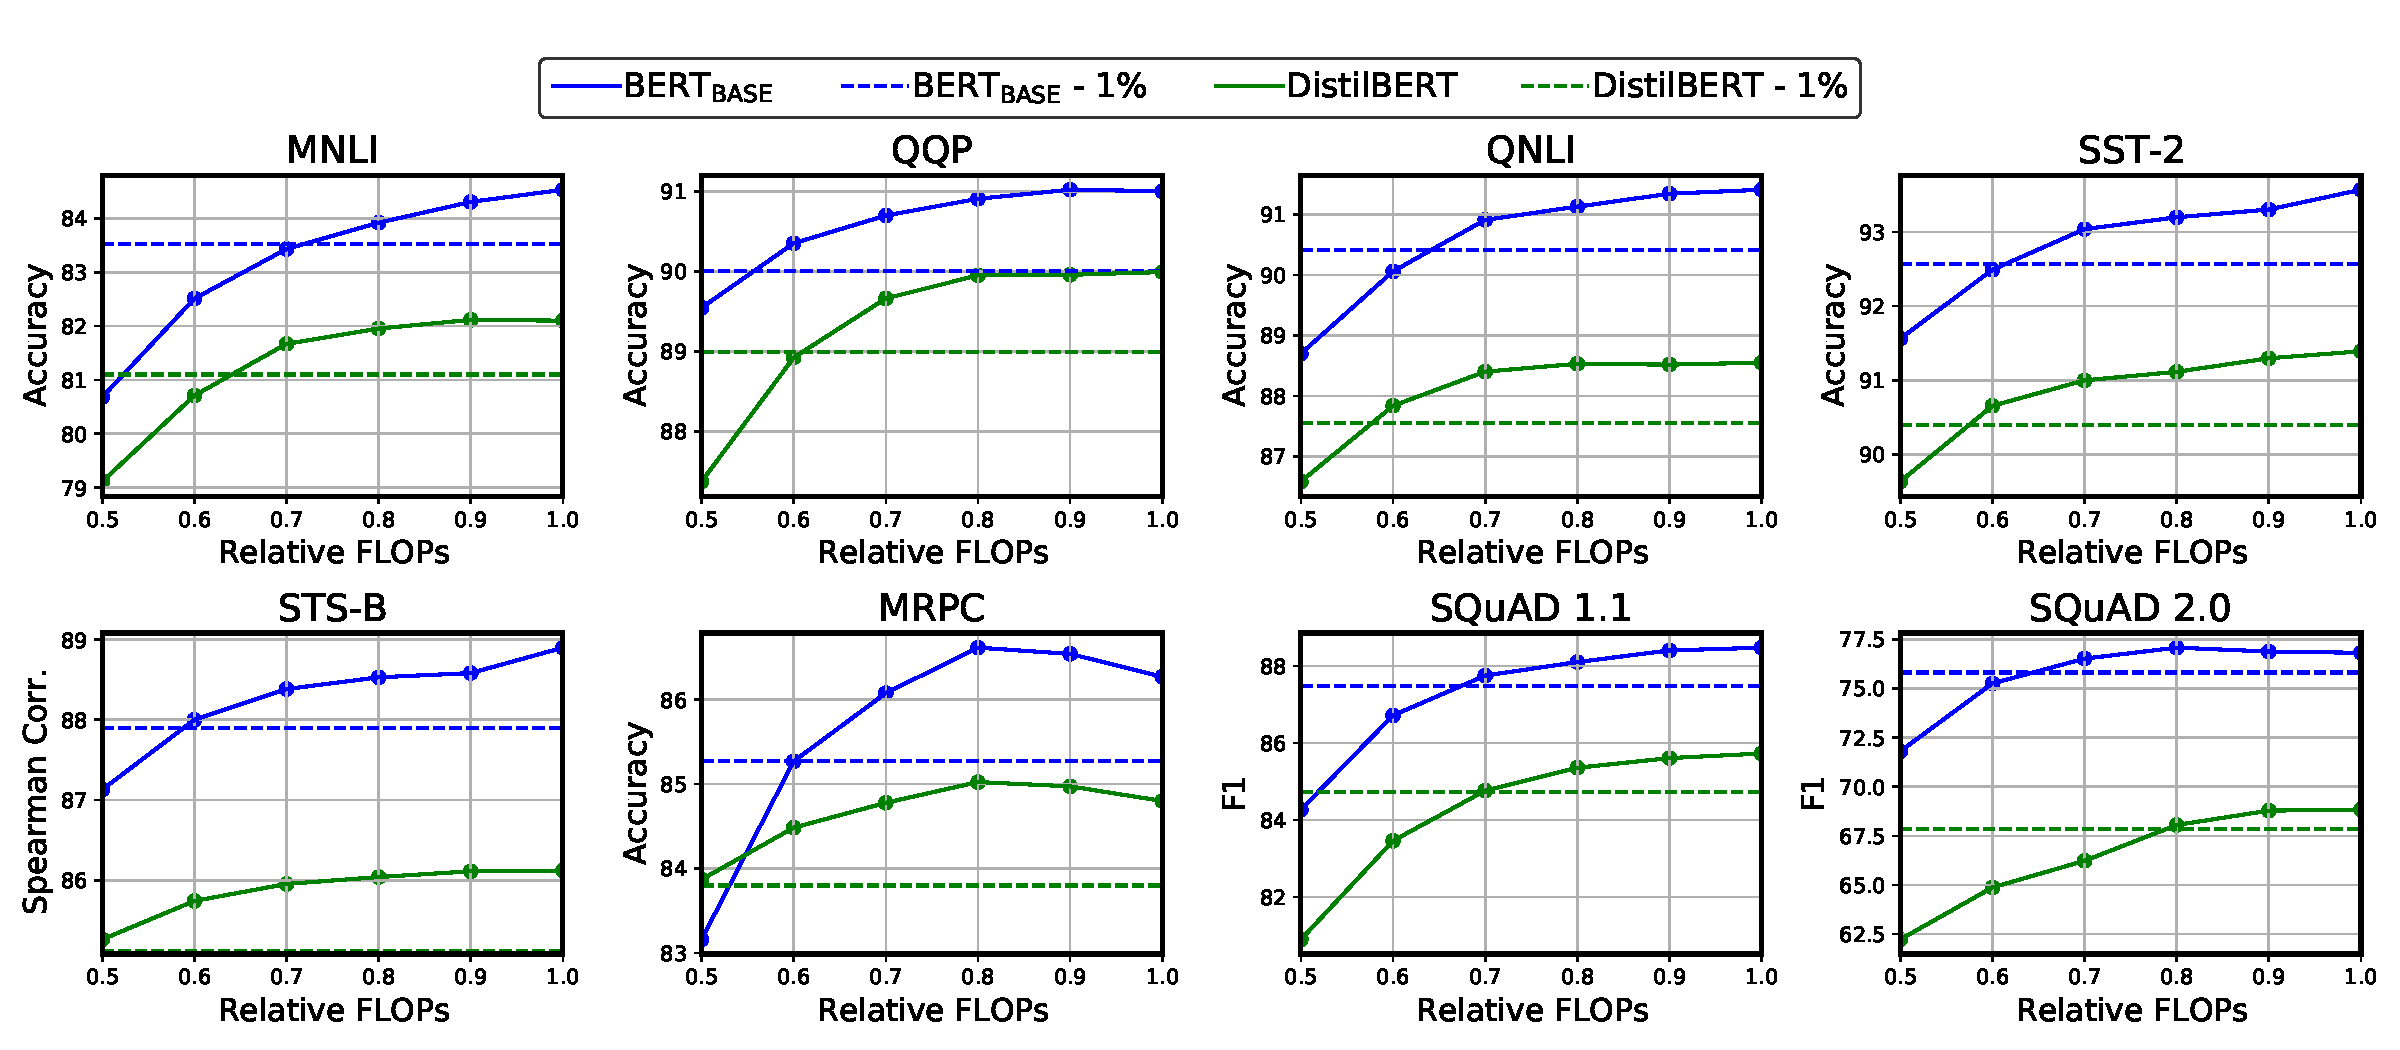
\includegraphics[width=\textwidth]{figures/flops.pdf}
\vspace{-7mm}
\caption{
Accuracy of our pruning method applied to BERT$_\textsc{BASE}$ and DistilBERT with different FLOPs constraints. 
The dashed horizontal lines indicate 1\% accuracy drop from the baseline models.
Note that these results can be achieved in only 39 and 135 seconds for GLUE and SQuAD benchmarks, respectively, on a single GPU system, as described in \tref{tab:time_breakdown} (in~\sref{appendix:time_breakdown}).
}
\vspace{-3mm}
\label{fig:flops_result}
\end{figure*}
%%%%%%%%%%%%%%%%%%%%%%%%%%%%%%%%%%%%%%%%%%%%%%%

%%%%%%%%%%%%%%%%%%%%%%%%%%%%%%%%%%%%%%%%%%%%%%%%%%%%%%%%%%%%%%%%%%%%%%%%%%%%%%
\begin{table*}[!t]
\caption{
Latency speedup of BERT$_\textsc{base}$ on a single NVIDIA V100 GPU with different batch sizes.
The latency is measured using PyTorch.
We constrain the accuracy degradation to be at most 1\% from the baseline accuracy,
and we report the largest speedup among those that satisfy the constraint.
}\label{tab:latency_result}
\vspace{-2mm}
\centerline{
    \centering
    \small{
    \setlength{\tabcolsep}{4.5pt}{
      \begin{tabular}{c|cccccccc|c}
        \toprule
        Batch size & {MNLI} & {QQP}  & {QNLI} & {SST-2} & {STS-B} & {MRPC} & {SQuAD$_{1.1}$} & {SQuAD$_{2.0}$} & Geo. mean\\ 
        \midrule         
        32 &  1.27$\times$ & 1.42$\times$ & 1.42$\times$ & 1.23$\times$ & 1.34$\times$ & 1.36$\times$ & 1.33$\times$ & 1.37$\times$ & 1.34$\times$ \\
        256 & 1.34$\times$ &	1.54$\times$ &	1.53$\times$ &	1.56$\times$ &	1.54$\times$ &	1.55$\times$ &	1.34$\times$ &	1.40$\times$ & 1.47$\times$\\
        \bottomrule
        \end{tabular} 
    }
    }
    % \vspace{-1mm}
}
\end{table*}
%%%%%%%%%%%%%%%%%%%%%%%%%%%%%%%%%%%%%%%%%%%%%%%%%%%%%%%%%%%%%%%%%%%%%%%%%%%%%%

% \vspace{-2mm}
\section{Evaluation}
\label{sec:eval}
\vspace{-1mm}

\subsection{Experimental Setup}
\label{subsection:experimental_setup}

Our framework is implemented on top of PyTorch~\cite{paszke2019pytorch} and the HuggingFace Transformers~\cite{wolf2020transformers} library.
We evaluate the effectiveness of our approach using BERT$_\textsc{BASE}$~\cite{devlin2018bert} and DistilBERT~\cite{sanh2019distilbert} on GLUE~\cite{wang2018glue} and SQuAD~\cite{rajpurkar2018know, rajpurkar2016squad} benchmarks.
We use 2K examples from the training sets for pruning, and we evaluate the resulting models on the development sets.
All of the results are averaged over the runs with 10 different seeds.
More details on the experimental setup can be found in \sref{appendix:eval_details}.


\subsection{Performance Evaluation}
\label{subsection:performance}

\textbf{FLOPs.} \fref{fig:flops_result} shows the accuracy of BERT$_\textsc{BASE}$ and DistilBERT with different
FLOPs constraints on GLUE and SQuAD datasets.
As can be seen in the plots, with only 1\% of accuracy drop, BERT$_\textsc{BASE}$ achieves 60--70\% of the original FLOPs  for all tasks. 
DistilBERT also shows a similar pattern and achieves up to 50\% FLOPs reduction (in STS-B and MRPC) even though it is already a compressed architecture.
More results using larger sample datasets are provided in~\sref{appendix:sample_dataset}.

\textbf{Latency.}
We further measure the latency on real hardware by pruning BERT$_\textsc{BASE}$ with latency constraints and deploying the resulting models on an NVIDIA V100 GPU.
\tref{tab:latency_result} lists the latency speedup with maximum accuracy drop of 1\% for GLUE and SQuAD datasets.
With batch size of 256, we achieve speedup of 1.47$\times$ on average and up to 1.56$\times$.

%%%%%%%%%%%%%%%%%%%%%%%%%%%%%%%%%%%%%%%%%%%%%%%
% \setlength{\textfloatsep}{0pt}
\begin{figure*}[!t]
% \vspace{-5mm}
\centering
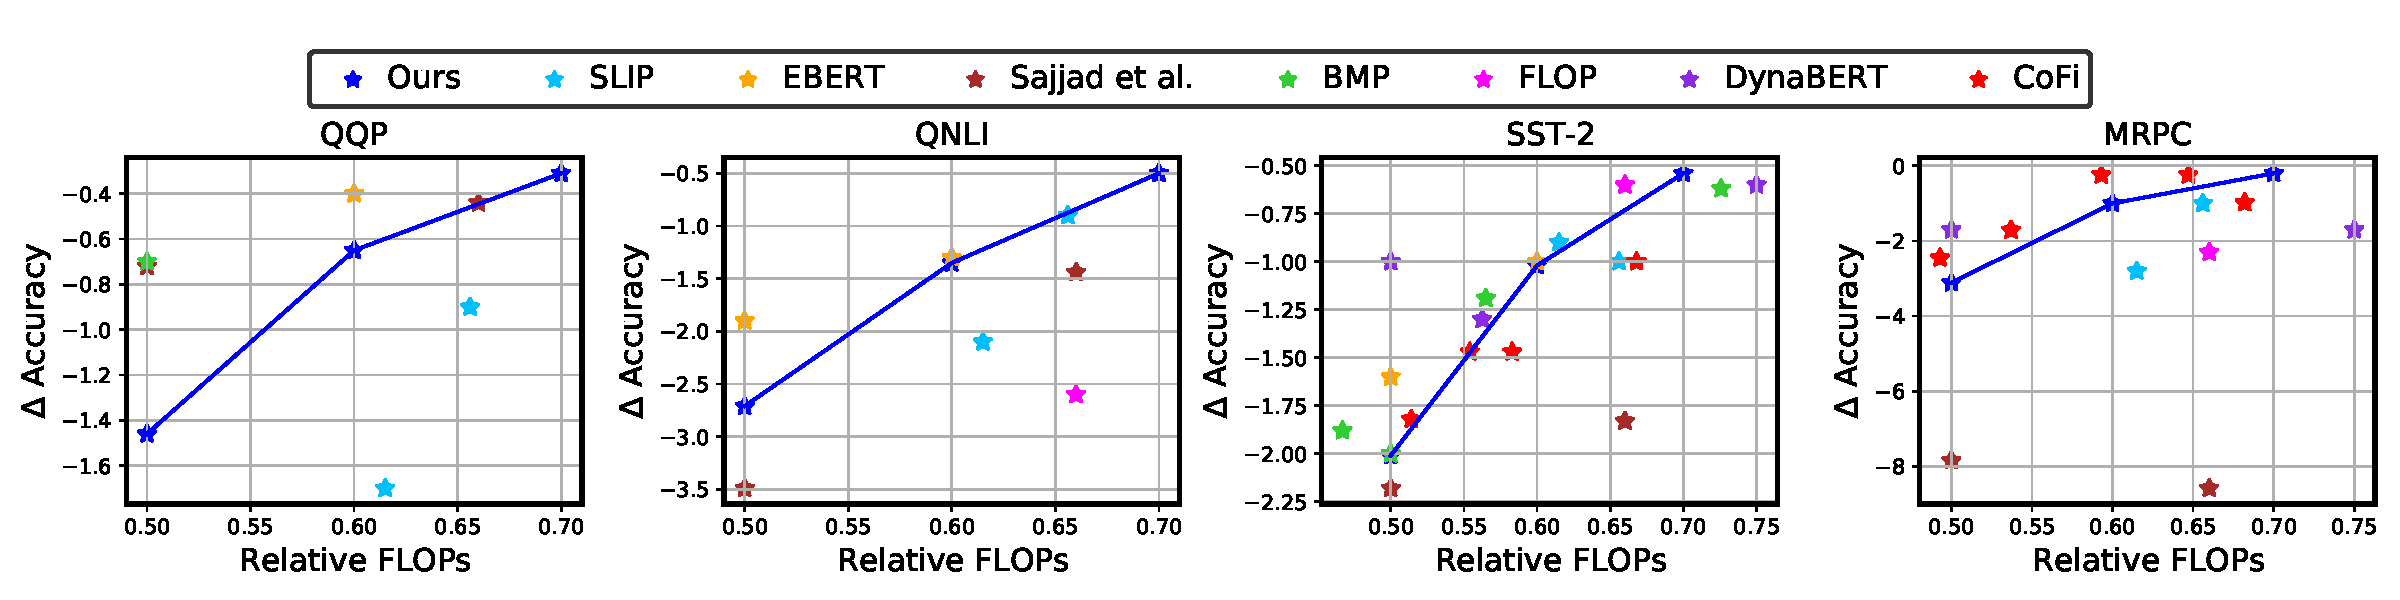
\includegraphics[width=1\textwidth]{figures/comparison.pdf}
% \vspace{-6mm}
\caption{
Amount of accuracy degradation from the baseline when pruning BERT$_\textsc{BASE}$ using our method and the prior structured pruning methods with different relative FLOPs. 
%without knowledge distillation and data augmentation techniques.
Note that our method does not require retraining, whereas all the other methods involve significant retraining overheads as described in \tref{tab:pruning_cost}.
}
% \vspace{-1mm}
\label{fig:comparison}
\end{figure*}
%%%%%%%%%%%%%%%%%%%%%%%%%%%%%%%%%%%%%%%%%%%%%%%

\subsection{Comparison with the Prior Methods}
\label{subsection:comparison}

\textbf{FLOPs and Accuracy Comparison.}
Here, we compare our method with the prior structured pruning methods for Transformers including 
Flop~\cite{wang2019structured}, 
SLIP~\cite{lin2020pruning}, 
Sajjad et al. \cite{sajjad2020effect}, 
DynaBERT~\cite{hou2020dynabert}, 
EBERT~\cite{liu2021ebert}, 
Block Movement Pruning (BMP)~\cite{lagunas2021block}, and CoFi~\cite{xia2022structured} by the FLOPs-accuracy trade-off of BERT$_\textsc{BASE}$ on GLUE tasks.
We use the results \textit{without} knowledge distillation and data augmentation reported in each paper. 
Since the baseline accuracy differs slightly from paper to paper, 
we compare the amount of the accuracy drop from the baseline instead of the absolute accuracy.
The results are plotted as~\fref{fig:comparison}.
We include the comparison details and full table in~\sref{appendix:comparison_details}.

Interestingly, our method exhibits comparable or better results than the prior methods \textit{without} any model retraining and with substantially lower pruning costs.
This empirically demonstrates that retraining and a complex pruning pipeline are \textit{not} necessary for moderate level of pruning of Transformers.
For high sparsity, we find that our framework \textit{with} retraining works comparably to or better than the prior methods at the same pruning cost (See~\sref{appendix:high_sparsity}).

%%%%%%%%%%%%%%%%%%%%%%%%%%%%%%%%%%%%%%%%%%%%%%%%%%%%%%%%%%%%%%%%%%%%%%%%%%%%%%
\begin{table}[!t]
	\begin{minipage}{0.47\linewidth}
	\vspace{-6mm}
		\centering
		\footnotesize
        \setlength{\tabcolsep}{3pt}
\caption{
Pruning cost comparison between the prior structured pruning methods and ours.
We compare the number of training epochs and the end-to-end (E2E) time required for pruning.
}
\vspace{2mm}
\label{tab:pruning_cost}
    \centering
    \small{
    \setlength{\tabcolsep}{5pt}{
       \begin{tabular}{lccc}
        \toprule
        & \# Epochs & E2E time (hr) \\ % & HP Free \\
        \midrule
        DynaBERT~\cite{hou2020dynabert} & 4 & 12 \\ %  & \red{\xmark}\\
        EBERT~\cite{liu2021ebert} & 6 & 5 \\ % & \red{\xmark} \\
        BMP~\cite{lagunas2021block} & 20 & 17 \\ % &  \red{\xmark} \\
        CoFi~\cite{xia2022structured} & 40 & 33 \\
        \midrule
        \ha Ours & \textbf{0} & \textbf{0.01} \\ % & \green{\cmark} \\
        \bottomrule
        \end{tabular} 
    }
    }
	\end{minipage}
	\hfill
	\begin{minipage}{0.52\linewidth}
  \begin{center}
    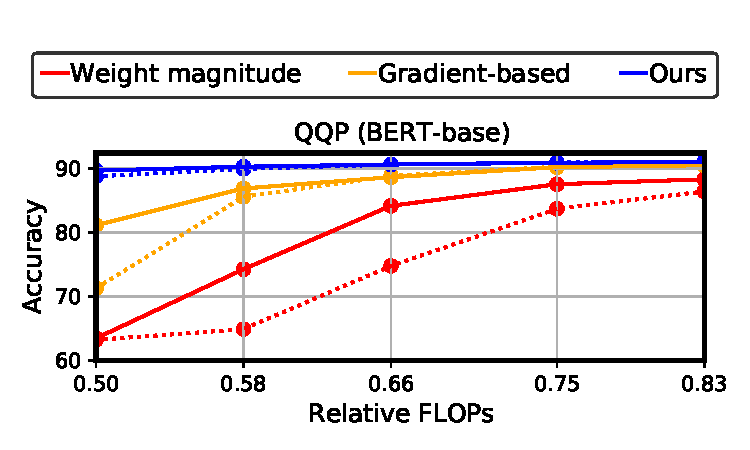
\includegraphics[width=1\columnwidth]{figures/effectiveness.pdf}
  \end{center}
  \vspace{-2mm}
  \captionof{figure}{
Retraining-free accuracy without (dotted) and with (solid) mask tuning.
}
\label{fig:effectiveness}
	\end{minipage}
	\vspace{-6mm}
\end{table}
%%%%%%%%%%%%%%%%%%%%%%%%%%%%%%%%%%%%%%%%%%%%%%%%%%%%%%%%%%%%%%%%%%%%%%%%%%%%%%


\textbf{Retraining Cost.}
We select DynaBERT~\cite{hou2020dynabert}, EBERT~\cite{liu2021ebert}, BMP~\cite{lagunas2021block}, and CoFi~\cite{xia2022structured} that achieve comparably good accuracy in \fref{fig:comparison}, and we systematically analyze their end-to-end retraining costs on MNLI dataset.
As shown in \tref{tab:pruning_cost}, these methods require 5$-$33 hours of retraining.
On the other hand, our method finishes in less than a minute, which is 2$-$3 orders of magnitude faster. 
We also highlight that this training latency analysis only accounts for a \textit{single} hyperparameter, and the entire cost should be multiplied by the size of the hyperparameter space.
While the prior methods rely on a considerable number of hyperparameters, ours introduce only two hyperparameters (in~\sref{subsec:tuning}) which we fix for all experiments.
See \sref{appendix:retraining_cost} for more details.

%%%%%%%%%%%%%%%%%%%%%%%%%%%%%%%%%%%%%%%%%%%%%%%%%%%%%%%%%%%%%%%%%%%%%%%%%%%%%%
\begin{table*}[!t]
\caption{
Ablation of our mask search, rearrangement, and tuning methods, described in \sref{sec:methodology}.
We use BERT$_\textsc{BASE}$ as the baseline model, and we prune it with a 60\% FLOPs constraint.
}
\vspace{-2mm}
% \vskip 0.05in
\label{tab:ablation}
    \centering
    \small{
    \setlength{\tabcolsep}{3pt}{
       \begin{tabular}{l|cccccccc|c}
        \toprule
         & {MNLI} & {QQP}  & {QNLI} & {SST-2} & {STS-B} & {MRPC} & {SQuAD$_{1.1}$} & {SQuAD$_{2.0}$} & {Avg. Diff} \\ 
        \midrule         
        Baseline & 84.53 &	91.00 &	91.41 &	93.57 &	88.90  & 86.27 & 88.48 &	76.82 & \\
        \midrule
        Mask Search & 81.21 &	89.99 &	88.38 &	92.13 &	87.10 & 83.14  &	82.66 &	71.12 & \\
        + Mask Rearrangement & 81.81 &	90.08 &	88.77 &	92.09 &	87.68 & 83.23  &	84.47 &	72.38 & + 0.60 \\
        \ha + Mask Tuning & \textbf{82.51} &	\textbf{90.35} &	\textbf{90.06} &	\textbf{92.49} &	\textbf{88.00} & \textbf{85.27}  &	\textbf{86.72} &	\textbf{75.26} & + 1.27 \\
        \bottomrule
        \end{tabular} 
    }
    }
\end{table*}
%%%%%%%%%%%%%%%%%%%%%%%%%%%%%%%%%%%%%%%%%%%%%%%%%%%%%%%%%%%%%%%%%%%%%%%%%%%%%%

\vspace{-1mm}
\subsection{Discussion} 
\label{subsection:analysis}
\vspace{-1mm}

\textbf{Ablation Studies.}
\tref{tab:ablation} lists an ablation of the mask rearrangement (\sref{subsec:rearrange}) and tuning (\sref{subsec:tuning}) stages for pruned BERT$_\textsc{base}$ with 60\% of FLOPs.
We find that both stages help recover the baseline accuracy, and that mask tuning is in particular critical, recovering up to 2.88\% accuracy.

To further investigate the importance of the mask search and rearrangement, we compare the \textit{retraining-free} performance of the binary masks obtained by our method and other pruning criteria: weight magnitude and the gradient-based method used in DynaBERT.
We uniformly pruned the layers using the two criteria with different width multipliers.
\fref{fig:effectiveness} shows that the two methods significantly degrade the accuracy under the low sparsity regimes.
Even with mask tuning, the accuracy is not fully recovered.
The results demonstrate that our mask search and re-arrangement are necessary to get optimal binary masks, and that mask tuning is only effective when the binary mask preserves high accuracy.
More ablation studies can be found in \sref{appendix:importance_metric} and \sref{appendix:abl-search-rearrange}.

\textbf{Time Breakdown.}
We break down our pruning pipeline into 4 parts---gradient computation, mask search, rearrangement, and tuning---and we measure the latency for each stage as \tref{tab:time_breakdown} (\sref{appendix:time_breakdown}).
For GLUE and SQuAD tasks, our framework finishes in 39 and 135 seconds on average.
